% Games: two-thirds of the average, and what a strategy actually is.
% Shared preamble for the write-on class slides.
%
% Every deck is designed to be projected and annotated live on a tablet:
% whatever takes time to draw is pre-drawn, and whatever the class produces is
% left blank. Compile a deck with `pdflatex main.tex` from its own directory,
% or run `make` in decks/ to build them all.
\documentclass[10pt]{article}

\usepackage[papersize={25.6cm,14.4cm}, margin=1.1cm, bottom=1.5cm,
            footskip=0.75cm]{geometry}
\usepackage[T1]{fontenc}
\usepackage[default]{sourcesanspro}
\usepackage{newtxsf}
\usepackage{tikz}
\usepackage{amsmath}
\usepackage{parskip}
\usepackage{fancyhdr}
\usetikzlibrary{arrows.meta, positioning, calc}

\setlength{\parindent}{0pt}

% Catppuccin Latte, the palette the course site uses in its light theme, so a
% deck on the projector looks like the pages the students read.
\definecolor{inkbg}{HTML}{EFF1F5}      % base
\definecolor{inksurface}{HTML}{E6E9EF} % mantle
\definecolor{inkfaint}{HTML}{CCD0DA}   % surface2, for rules and empty boxes
\definecolor{inktext}{HTML}{4C4F69}    % text
\definecolor{inkgrey}{HTML}{8C8FA1}    % overlay1, for anything secondary
\definecolor{inkblue}{HTML}{7287FD}    % lavender, the primary accent
\definecolor{inkteal}{HTML}{179299}    % teal
\definecolor{inkred}{HTML}{FE640B}     % peach, for whatever wants attention
\definecolor{inkmauve}{HTML}{8839EF}   % mauve

\pagecolor{inkbg}
\color{inktext}

% A box to write a number into. White against the tinted page, so it reads as
% somewhere to write rather than as part of the printed material.
\newcommand{\blank}[1][1.6]{%
  \tikz[baseline=(current bounding box.base)]{%
    \draw[inkfaint, line width=0.7pt, rounded corners=2pt, fill=white]
      (0,-0.18) rectangle (#1,0.62);}}

% A ruled area to work in. Faint dots keep handwriting level on a tablet.
\newcommand{\workspace}[2]{%
  \begin{tikzpicture}
    \draw[inkfaint, line width=0.7pt, rounded corners=3pt, fill=white]
      (0,0) rectangle (#1,#2);
    \foreach \gx in {0.5,1.0,...,#1}{%
      \foreach \gy in {0.5,1.0,...,#2}{%
        \fill[inkfaint] (\gx,\gy) circle (0.5pt);}}
  \end{tikzpicture}}

% A panel for material that is printed rather than written on.
\newcommand{\panel}[2]{%
  \begin{tikzpicture}
    \draw[inkfaint, line width=0.7pt, rounded corners=3pt, fill=inksurface]
      (0,0) rectangle (#1,#2);
  \end{tikzpicture}}

% An empty payoff grid. #1 is the list of action names, #2 is drawn afterwards
% so a page can add its own marks.
\newcommand{\payoffgrid}[2]{%
  \begin{tikzpicture}[scale=1.0, every node/.style={transform shape}]
    \foreach \name [count=\j from 0] in {#1}{%
      \node[font=\bfseries, text=inkblue] at (\j*2.7+1.35,0.55) {\name};
      \node[font=\bfseries, text=inkblue] at (-1.15,-\j*2-1) {\name};
      \foreach \k [count=\i from 0] in {#1}{%
        \draw[inkfaint, line width=0.7pt, fill=white]
          (\j*2.7,-\i*2) rectangle (\j*2.7+2.7,-\i*2-2);}}
    #2
  \end{tikzpicture}}

% The five actions on a pentagon. Each action beats the one next to it and the
% one across from it, so the two winning cycles are drawn as separate panels:
% ten labelled arrows on one diagram is a tangle nobody can read from the back
% of the room.
\newcommand{\rpslscycle}[3]{%
  \begin{tikzpicture}[scale=1.0, every node/.style={transform shape},
      >={Stealth[length=2.6mm]},
      action/.style={circle, draw=inkfaint, line width=1pt, fill=white,
                     text=inktext, minimum size=1.7cm, inner sep=1pt,
                     font=\small\bfseries},
      beats/.style={->, line width=1.2pt, shorten >=3pt, shorten <=3pt,
                    draw=#1},
      word/.style={font=\scriptsize, fill=inkbg, inner sep=1.6pt, text=#1,
                   sloped, pos=#2}]
    \foreach \name/\angle in {Rock/90, Lizard/18, Spock/-54,
                              Scissors/-126, Paper/162}{%
      \node[action] (\name) at (\angle:3.1) {\name};}
    \foreach \winner/\loser/\said in {#3}{%
      \draw[beats] (\winner) -- node[word] {\said} (\loser);}
  \end{tikzpicture}}

% Running header: the deck name on the left, the page's own step on the right.
% Each deck sets its name once with \deckname.
\newcommand{\deck}{}
\newcommand{\deckname}[1]{\renewcommand{\deck}{#1}}
\newcommand{\slidehead}[1]{%
  {\small\color{inkgrey}%
   \tikz[baseline=-0.5ex]{\fill[inkblue, rounded corners=1pt]
     (0,0) rectangle (0.22,0.22);}\;\deck
   \hfill \color{inkblue}\bfseries #1}\par
  {\color{inkblue}\rule{\linewidth}{1pt}}\par\vspace{0.35em}}

\pagestyle{fancy}
\fancyhf{}
\renewcommand{\headrulewidth}{0pt}
\fancyfoot[R]{\small\color{inkgrey}\thepage}

% Deck title pages, which carry no header and no page number.
\newcommand{\titleslide}[3]{%
  \thispagestyle{empty}%
  \begin{center}
    \vspace*{\fill}
    {\Huge\bfseries\color{inkblue} #1}\\[0.7em]
    {\LARGE\color{inkgrey} #2}\\[2.4em]
    #3
    \vspace*{\fill}
  \end{center}}

% One step of the plan on a title page.
\newcommand{\stepbox}[3]{%
  \node[draw=inkblue, line width=0.9pt, rounded corners=4pt, fill=white,
        minimum width=6cm, minimum height=1.7cm, align=center,
        text=inktext] (#1) at (#2,0) {#3};}


% Blank axes for sketching the class's Menti distribution.
\newcommand{\distribution}{%
  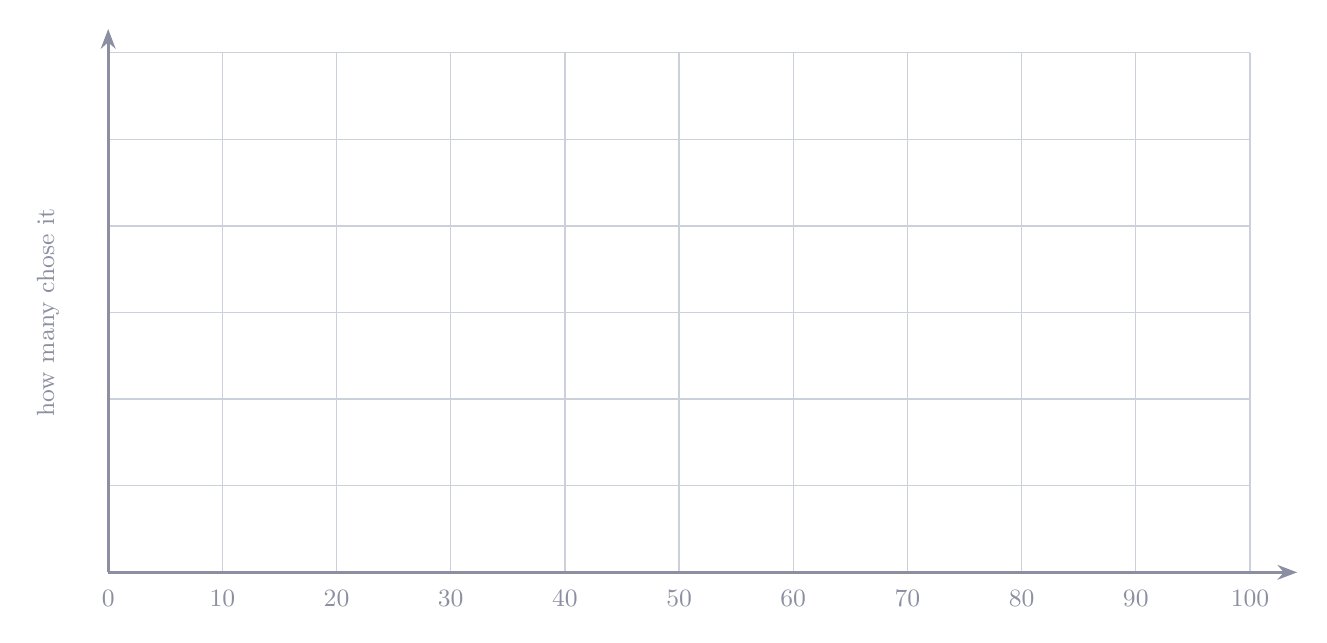
\begin{tikzpicture}[scale=1.0, every node/.style={transform shape}]
    \fill[white] (0,0) rectangle (14.5,6.6);
    \foreach \x in {0,10,...,100}{%
      \draw[inkfaint, line width=0.5pt] (\x*0.145,0) -- (\x*0.145,6.6);}
    \foreach \y in {1,2,3,4,5,6}{%
      \draw[inkfaint, line width=0.5pt] (0,\y*1.1) -- (14.5,\y*1.1);}
    \draw[inkgrey, line width=1pt, -{Stealth[length=2.5mm]}] (0,0) -- (15.1,0);
    \draw[inkgrey, line width=1pt, -{Stealth[length=2.5mm]}] (0,0) -- (0,6.9);
    \foreach \x in {0,10,...,100}{%
      \node[below, font=\small, text=inkgrey] at (\x*0.145,-0.1) {\x};}
    \node[left, font=\small, text=inkgrey, rotate=90, anchor=south]
      at (-0.5,3.3) {how many chose it};
  \end{tikzpicture}}

\deckname{Games}

\begin{document}

\titleslide{Games}{Two thirds of the average, twice}{%
    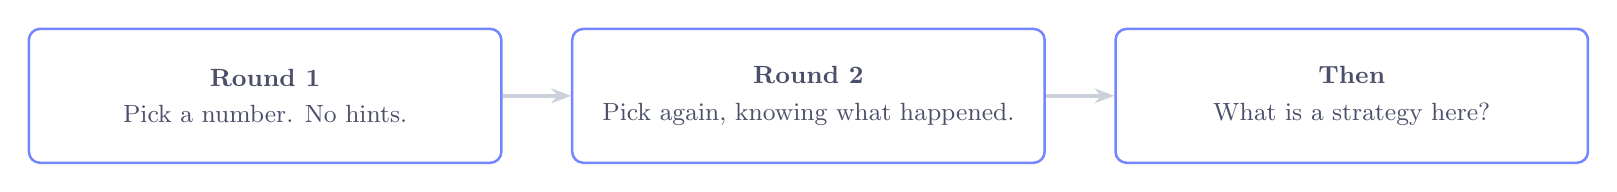
\begin{tikzpicture}[font=\small]
      \stepbox{s0}{0.0}{\textbf{Round 1}\\[0.25em] Pick a number. No hints.}
      \stepbox{s1}{6.9}{\textbf{Round 2}\\[0.25em] Pick again, knowing what happened.}
      \stepbox{s2}{13.8}{\textbf{Then}\\[0.25em] What is a strategy here?}
      \draw[-{Stealth[length=2.5mm]}, inkfaint, line width=1.2pt] (s0) -- (s1);
      \draw[-{Stealth[length=2.5mm]}, inkfaint, line width=1.2pt] (s1) -- (s2);
    \end{tikzpicture}

    \vspace{2.4em}

    {\large Pick a whole number between 0 and 100. Closest to two thirds of
   the average wins.}}

\newpage
\slidehead{Round 1}

\vspace{0.1cm}

\begin{minipage}[c]{0.71\linewidth}
\distribution
\end{minipage}
\hfill
\begin{minipage}[c]{0.25\linewidth}
{\large
Average\\[0.4em]
\hspace*{0.3cm}\blank[2.4]\\[1.5em]
Two thirds of it\\[0.4em]
\hspace*{0.3cm}\blank[2.4]\\[1.5em]
Winner\\[0.4em]
\hspace*{0.3cm}\blank[2.4]}
\end{minipage}

\newpage
\slidehead{Why would you go lower?}

\vspace{0.9cm}

\begin{center}
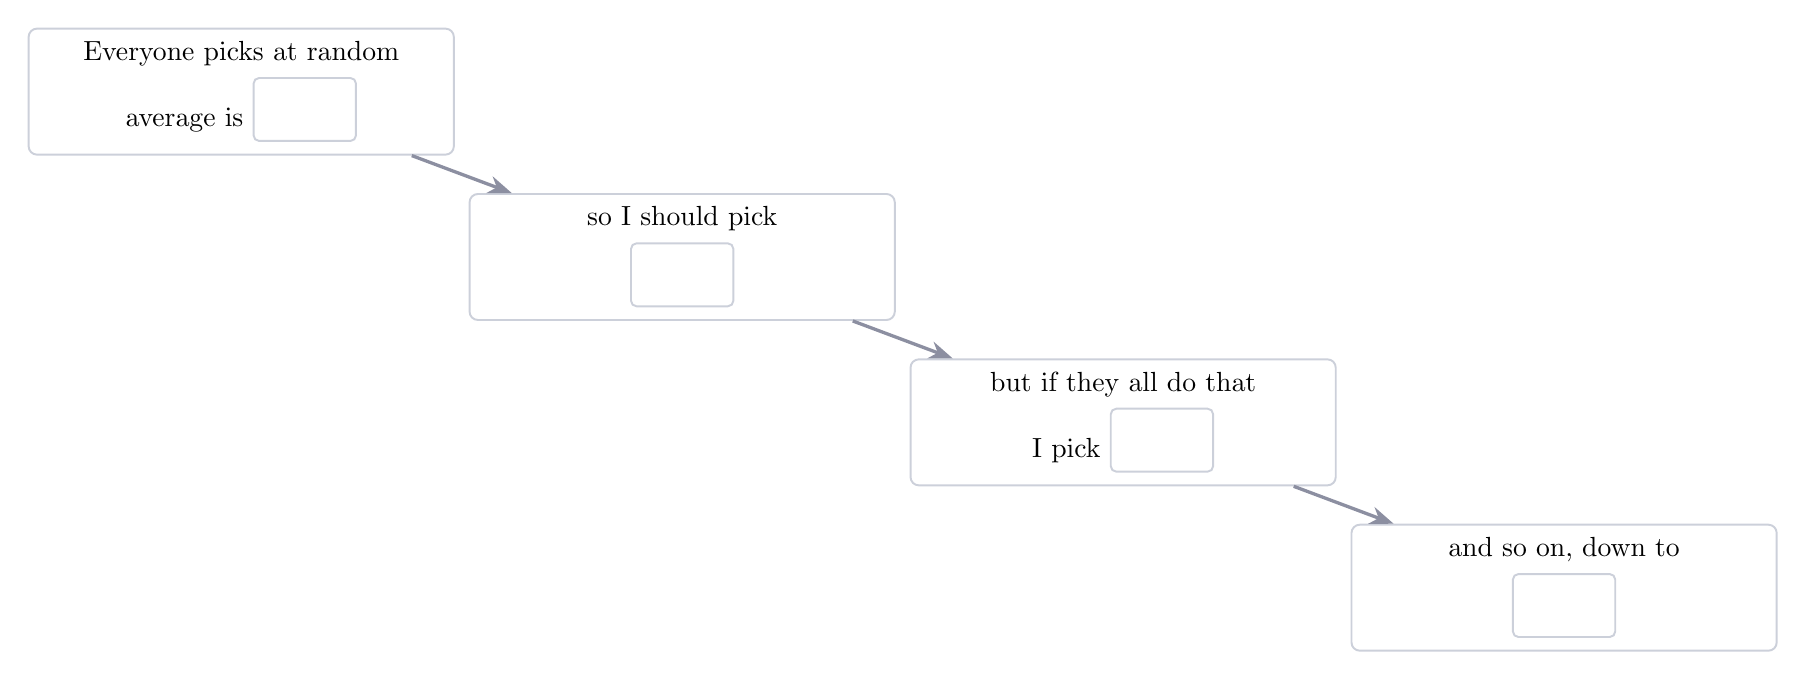
\begin{tikzpicture}[font=\large,
    rung/.style={draw=inkfaint, line width=0.7pt, rounded corners=3pt,
                 minimum width=5.4cm, minimum height=1.6cm, align=center,
                 font=\normalsize}]
  \node[rung] (l0) at (0,0)
    {Everyone picks at random\\[0.3em] average is \blank[1.3]};
  \node[rung] (l1) at (5.6,-2.1)
    {so I should pick\\[0.3em] \blank[1.3]};
  \node[rung] (l2) at (11.2,-4.2)
    {but if they all do that\\[0.3em] I pick \blank[1.3]};
  \node[rung] (l3) at (16.8,-6.3)
    {and so on, down to\\[0.3em] \blank[1.3]};
  \draw[-{Stealth[length=3mm]}, inkgrey, line width=1.2pt] (l0) -- (l1);
  \draw[-{Stealth[length=3mm]}, inkgrey, line width=1.2pt] (l1) -- (l2);
  \draw[-{Stealth[length=3mm]}, inkgrey, line width=1.2pt] (l2) -- (l3);
\end{tikzpicture}
\end{center}

\vspace{0.5cm}

{\large How far down the ladder did the room actually go? \blank[2.4] steps.}

\newpage
\slidehead{Round 2}

\vspace{0.1cm}

\begin{minipage}[c]{0.71\linewidth}
\distribution
\end{minipage}
\hfill
\begin{minipage}[c]{0.25\linewidth}
{\large
Average\\[0.4em]
\hspace*{0.3cm}\blank[2.4]\\[1.5em]
Two thirds of it\\[0.4em]
\hspace*{0.3cm}\blank[2.4]\\[1.5em]
Winner\\[0.4em]
\hspace*{0.3cm}\blank[2.4]}
\end{minipage}

\newpage
\slidehead{Which kind of game is this?}

\vspace{0.7cm}

\begin{minipage}[t]{0.47\linewidth}
{\large\bfseries Normal form}

\vspace{0.5em}

{\large Everyone chooses \underline{\hspace{3.5cm}}, and a payoff
follows.}

\vspace{0.8em}

\workspace{10.6}{4.4}
\end{minipage}
\hfill
\begin{minipage}[t]{0.47\linewidth}
{\large\bfseries Extensive form}

\vspace{0.5em}

{\large Players move \underline{\hspace{3.5cm}}, and can see what has
happened.}

\vspace{0.8em}

\workspace{10.6}{4.4}
\end{minipage}

\vspace{0.9cm}

{\large Our game is \underline{\hspace{5cm}}, because
\underline{\hspace{7cm}}.}

\newpage
\slidehead{So what is a strategy?}

\vspace{0.8cm}

{\large In the game we just played, a strategy is
\underline{\hspace{9cm}}.}

\vspace{1.1cm}

{\large Now change the rules: you pick \emph{after} hearing what the person
before you picked. Draw a couple of levels of that game.}

\vspace{0.7cm}

\begin{center}
\workspace{22.6}{4.6}
\end{center}

\vspace{0.5cm}

{\large In \emph{that} game, a strategy has to say \blank[6].}

\newpage
\slidehead{The same thing, as an exam answer}

\vspace{0.9cm}

{\large This material is not examined on its own. Normal form, extensive form,
strategies and best responses are examined together with \textbf{Nash
Equilibrium}, so the natural follow-up is \textbf{Question 1} on that page.}

\vspace{1.2cm}

{\large The habit worth building now: whenever we play something, ask what the
players, the actions and the payoffs are, and write them down before doing any
algebra.}

\vspace{1.6cm}

\begin{center}
{\large\color{inkgrey} vknight.org/gt/topics/nash-equilibrium.html}
\end{center}

\end{document}
